\documentclass[10pt]{article}
\usepackage[italian]{babel}
\usepackage[utf8]{inputenc}
\usepackage[T1]{fontenc}
\usepackage{graphicx}
\usepackage[export]{adjustbox}
\graphicspath{ {./images/} }
\usepackage{amsmath}
\usepackage{amsfonts}
\usepackage{amssymb}
\usepackage[version=4]{mhchem}
\usepackage{stmaryrd}

\usepackage{float}

\usepackage{titling}
\pretitle{\begin{center}
\includegraphics[width=\textwidth]{/home/keyser/Coding/cosmesi_ale/cose da aggiungere/header_WATT+}\\[6em]}
	\posttitle{\end{center}}  

\title{\Huge{MANUALE COPERTA SAUNA A INFRAROSSI}}

\author{}
\date{}


\begin{document}
	
\maketitle

\begin{figure}[H]
	\centering
	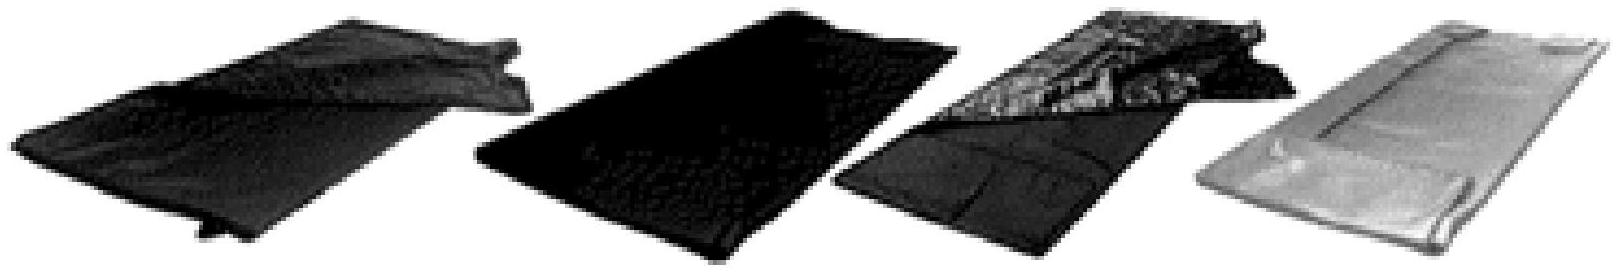
\includegraphics[width=\textwidth]{db2c8f34-1479-42f9-a6f5-45da4ab45a37-1_275_1620_868_219}
\end{figure}

\newpage

\tableofcontents

\section{Manuale di istruzioni}

Questo è il manuale originale.\\
Si prega di leggere attentamente tutte le istruzioni prima dell'uso.\\
L'aspetto del prodotto può differire leggermente in base al modello ricevuto.\\
L'azienda non informerà l'utente in caso di aggiornamenti tecnologici o software del prodotto.

\section{AVVERTENZE DI SICUREZZA}
\begin{enumerate}
  \item Tenere fuori dalla portata dei bambini.
  \item Attendere almeno 30 minuti dopo i pasti prima dell'uso.
  \item Usare solo il cavo di alimentazione fornito, alla tensione e frequenza indicate. Non usare cavi non originali.
  \item Non lasciare mai il dispositivo incustodito quando è collegato o in funzione. Dopo l'uso scollegarlo e lasciarlo raffreddare prima di pulizia, stoccaggio o spostamento.
  \item Spegnere e scollegare dalla rete quando non viene utilizzato per lunghi periodi.
  \item Non usare in ambienti umidi. Non bagnare la centralina o i cavi. Non immergere in acqua. Se la centralina si bagna o emette odore, scollegare immediatamente.
  \item Non piegare la coperta e non appoggiare oggetti pesanti mentre è in funzione.
  \item Non posizionare la centralina sulla coperta in funzione per evitare surriscaldamenti o fusione dei componenti.
  \item Non usare vicino a fornelli elettrici o fonti di calore elevate.
  \item Usare solo su superfici resistenti al calore.
  \item Non usare su letti ad acqua, lattice, plastica, memory foam, reti regolabili, letti a castello, lettini per bambini o materiali sintetici o infiammabili.
  \item Non avvolgere i cavi strettamente intorno al tappetino o alla centralina.
  \item Conservare in luogo asciutto e lontano dalla luce solare diretta.
  \item Pulire con un panno morbido dopo ogni utilizzo.
  \item Evitare il contatto con oggetti taglienti o duri.
  \item Non usare o conservare all'aperto.
  \item Non usare durante temporali o fulmini.
  \item Se il dispositivo emette rumori anomali, spegnere e scollegare immediatamente.
\end{enumerate}

\section{TEMPO DI PRERISCALDAMENTO}
Si consiglia di entrare nella coperta $3-5$ minuti dopo l'accensione.\\
Il riscaldamento completo richiede circa 15 minuti (soprattutto in inverno o nei paesi a 110 V).

\section{CENTRALINA TOUCHSCREEN}
\begin{center}
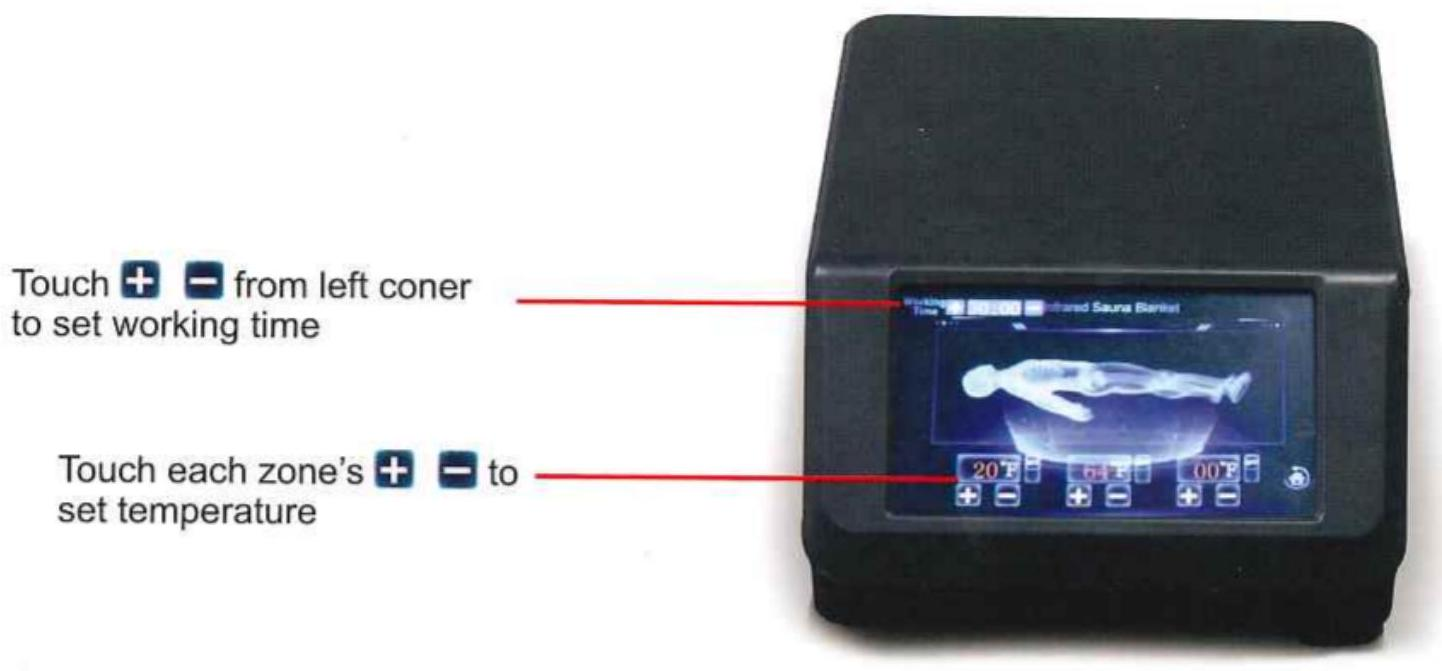
\includegraphics[max width=\textwidth, alt={}]{db2c8f34-1479-42f9-a6f5-45da4ab45a37-3_671_1442_1162_251}
\end{center}

\begin{enumerate}
  \item Collegare
  \item Premere ENTER
  \item Toccare per impostare tempo e temperatura
  \item Premere ON
  \item A fine ciclo premere HOME sullo schermo e scollegare
\end{enumerate}

Specifiche D + E

\begin{itemize}
  \item Dimensioni: $180 \times 190 \mathrm{~cm}$
  \item Peso netto: $10,5 \mathrm{~kg}$, Peso Lordo $11,5 \mathrm{Kg}$
  \item Dimesioni: $52 \times 23 \times 46 \mathrm{~cm}$
  \item Alimentazione:\\
$-110 \mathrm{~V}-450 \mathrm{~W} ; 60 \mathrm{~Hz}$\\
$-220 \mathrm{~V}-560 \mathrm{~W} ; 50 \mathrm{~Hz}$
\end{itemize}

\newpage

% --- INIZIO INFORMATIVA PRIVACY ---
\newpage

\section{INFORMATIVA PRIVACY}
\begin{center}
	(ai sensi dell'art. 13 del Regolamento UE 2016/679)
\end{center}

La presente informativa è resa ai sensi del Regolamento Generale sulla Protezione dei Dati (GDPR) e riguarda il trattamento dei dati personali dei clienti che si sottopongono a trattamenti e tecnologie estetiche.

\subsection*{Titolare del trattamento}

Il Titolare del trattamento è:

\begin{itemize}
	\item Denominazione centro estetico: \underline{\hspace{5cm}}
	\item Sede legale: \underline{\hspace{7cm}}
	\item P. IVA / C.F.: \underline{\hspace{6cm}}
	\item Contatti (telefono/email): \underline{\hspace{5cm}}
\end{itemize}

\subsection*{Tipologia di dati trattati}

Il Titolare può raccogliere e trattare le seguenti categorie di dati:

\begin{itemize}
	\item Dati anagrafici (nome, cognome, data di nascita)
	\item Dati di contatto (telefono, e-mail)
	\item Dati fiscali per eventuale fatturazione
	\item Dati particolari relativi allo stato di salute (allergie, patologie, gravidanza, terapie in corso) necessari per valutare l'idoneità ai trattamenti estetici
	\item Eventuali immagini fotografiche prima/dopo trattamento (previo consenso specifico)
\end{itemize}

\subsection*{Finalità del trattamento}

I dati personali sono trattati per le seguenti finalità:

\begin{enumerate}
	\item Esecuzione di trattamenti estetici e utilizzo di tecnologie professionali (laser, radiofrequenza, ultrasuoni, pressoterapia, ecc.)
	\item Valutazione dell'idoneità al trattamento
	\item Adempimenti amministrativi, contabili e fiscali
	\item Gestione degli appuntamenti
	\item Eventuale invio di comunicazioni promozionali (solo previo consenso separato)
	\item Eventuale utilizzo di immagini per finalità informative o promozionali (solo previo consenso separato)
\end{enumerate}

\subsection*{Base giuridica del trattamento}

Il trattamento dei dati si fonda su:

\begin{itemize}
	\item Esecuzione del contratto/prestazione richiesta
	\item Adempimento di obblighi di legge
	\item Consenso esplicito dell'interessato per il trattamento di dati particolari (sanitari)
	\item Consenso separato per marketing e utilizzo immagini
\end{itemize}

\subsection*{Modalità di trattamento}

Il trattamento dei dati avviene mediante strumenti cartacei e/o informatici, nel rispetto dei principi di correttezza, liceità, trasparenza e tutela della riservatezza.

Sono adottate adeguate misure di sicurezza per prevenire accessi non autorizzati, perdita o diffusione dei dati.

\subsection*{Conservazione dei dati}

I dati personali saranno conservati:

\begin{itemize}
	\item Per il tempo necessario all'erogazione del servizio
	\item Per il periodo previsto dalla normativa fiscale e civilistica
	\item Fino a revoca del consenso per finalità di marketing o utilizzo immagini
\end{itemize}

\subsection*{Comunicazione dei dati}

I dati potranno essere comunicati a:

\begin{itemize}
	\item Consulenti fiscali e amministrativi
	\item Software gestionali utilizzati per la gestione clienti
	\item Autorità competenti, ove previsto dalla legge
\end{itemize}

I dati non saranno diffusi senza consenso.

\subsection*{Diritti dell'interessato}

L'interessato può esercitare in qualsiasi momento i seguenti diritti:

\begin{itemize}
	\item Accesso ai propri dati
	\item Rettifica o aggiornamento
	\item Cancellazione (diritto all'oblio)
	\item Limitazione del trattamento
	\item Opposizione al trattamento
	\item Revoca del consenso
	\item Reclamo all'Autorità Garante per la Protezione dei Dati Personali
\end{itemize}

Le richieste possono essere inviate ai recapiti del Titolare sopra indicati.

\subsection*{Natura del conferimento dei dati}

Il conferimento dei dati è necessario per l'erogazione dei trattamenti estetici.
Il mancato conferimento può comportare l'impossibilità di eseguire il servizio.

\subsection*{CONSENSO}

Il/La sottoscritto/a dichiara di aver ricevuto e compreso la presente informativa.

\vspace{0.8cm}

Data: \underline{\hspace{5cm}} 

\vspace{15pt}
Firma: \underline{\hspace{6cm}}

\vspace{1cm}

$\square$ Acconsento al trattamento dei dati particolari (sanitari)

\vspace{0.3cm}
$\square$ Acconsento all'utilizzo delle immagini per finalità promozionali

\vspace{0.3cm}
$\square$ Acconsento a ricevere comunicazioni promozionali

% --- FINE INFORMATIVA PRIVACY ---

\newpage


\begin{figure}[H]
	\centering
	\includegraphics[width=0.7\paperwidth,height=\paperheight, keepaspectratio]{"../cose da aggiungere/privacy_conformita/dichiarazione_conformita"}
\end{figure}


\section{Simboli}
\begin{figure}[H]
	\centering
	
\includegraphics[width=\linewidth]{pittogrammi_1}
%	\caption{}
	\label{fig:pittogrammi1}
\end{figure}
\begin{figure}[H]
	\centering
	
\includegraphics[width=\linewidth]{pittogrammi_2}
%	\caption{}
	\label{fig:pittogrammi2}
\end{figure}
\begin{figure}[H]
	\centering
	
\includegraphics[width=\linewidth]{pittogrammi_3}
%	\caption{}
	\label{fig:pittogrammi3}
\end{figure}
\begin{figure}[H]
	\centering
	
\includegraphics[width=\linewidth]{pittogrammi_4}
%	\caption{}
	\label{fig:pittogrammi4}
\end{figure}
\begin{figure}[H]
	\centering
	
\includegraphics[width=\linewidth]{pittogrammi_5}
%	\caption{}
	\label{fig:pittogrammi5}
\end{figure}


\end{document}